\documentclass{article}
\usepackage[utf8]{inputenc}
\usepackage[margin=0.5in,includefoot]{geometry}
\usepackage[export]{adjustbox}

% Header and Footer Setup
\usepackage{fancyhdr}
\pagestyle{fancy}
\fancyhead{}
\fancyfoot{}
\fancyfoot[R]{\thepage}
\renewcommand{\headrulewidth}{0pt}
\renewcommand{\footrulewidth}{0pt}
%
%Graphics Setup
\usepackage{graphicx}
\usepackage{float}
\usepackage{subfig}


%list setup
\usepackage{amssymb}
\renewcommand{\labelitemi}{$\blacktriangleright$}
\renewcommand{\labelitemii}{$\bullet$}
\renewcommand{\labelitemiii}{$\circ$}

%Source Code setup
\usepackage{xcolor}
\usepackage{listings}

\definecolor{mGreen}{rgb}{0,0.6,0}
\definecolor{mGray}{rgb}{0.5,0.5,0.5}
\definecolor{mPurple}{rgb}{0.58,0,0.82}
\definecolor{backgroundColour}{rgb}{0.95,0.95,0.92}

\lstdefinestyle{CStyle}{
    backgroundcolor=\color{backgroundColour},   
    commentstyle=\color{mGreen},
    keywordstyle=\color{magenta},
    numberstyle=\tiny\color{mGray},
    stringstyle=\color{mPurple},
    basicstyle=\footnotesize,
    breakatwhitespace=false,         
    breaklines=true,                 
    captionpos=b,                    
    keepspaces=true,                 
    numbers=left,                    
    numbersep=5pt,                  
    showspaces=false,                
    showstringspaces=false,
    showtabs=false,                  
    tabsize=2,
    language=C
}
%


\begin{document}

\begin{titlepage}

	\begin{flushright}
	\textsc{\large May 3, 2021} \\
	\end{flushright}
	\begin{center}
	\Large{\bfseries GTU Department of Computer Engineering \\ CSE344 - Spring 2021 \\ Midterm Report  } \\
	\end{center}
	\topskip0pt
	\vspace*{\fill}
	\begin{center}
	\Large{\bfseries Akif Kartal \\ 171044098 }
	\end{center}
	\vspace*{\fill}

\end{titlepage}

\cleardoublepage
\section{Problem Definition}
The problem is to implement \textbf{producer-consumer} problem by simulating covid19
vaccination flow by using shared memory and posix semaphore. 

\section{Solution}
The homework was finished as expected in homework pdf file. 
\subsection{Some Problems and Solutions}
\subsubsection{Semaphore Usage}
In order to provide synchronization between processes I used \textbf{7 posix named semaphore}.
Followings are my semaphores;
\begin{lstlisting}[style=CStyle]
    /*create named semphores*/
    sem_mutex = sem_open("mutex344", O_CREAT, 0666, 1);
    if (sem_mutex == SEM_FAILED)
        errExit("sem_open error!");

    sem_vac = sem_open("wait_vaccinator", O_CREAT, 0666, 0);
    if (sem_vac == SEM_FAILED)
        errExit("sem_open error!");

    sem_cit = sem_open("wait_citizen", O_CREAT, 0666, 0);
    if (sem_cit == SEM_FAILED)
        errExit("sem_open error!");

    sem_full1 = sem_open("full344", O_CREAT, 0666, 0);
    if (sem_full1 == SEM_FAILED)
        errExit("sem_open error!");
    sem_empty = sem_open("empty344", O_CREAT, 0666, bufferSize);
    if (sem_empty == SEM_FAILED)
        errExit("sem_open error!");
    sem_full2 = sem_open("full3442", O_CREAT, 0666, 0);
    if (sem_full2 == SEM_FAILED)
        errExit("sem_open error!");
    sem_run = sem_open("whorunfirst", O_CREAT, 0666, 0);
    if (sem_run == SEM_FAILED)
        errExit("sem_open error!");
\end{lstlisting}
Usage purpose of each semaphore will be explained in detail coming pages.
\subsubsection{Shared Memory Usage}
In order to use shared memory correct way between process I made following struct to keep in shared memory for each process.
Note that this memory is generic between all process.
\begin{lstlisting}[style=CStyle]
typedef struct GTU344
{
    args givenParams;
    int dose1;
    int dose2;
    int totalLeft;
    int isRead;
    int fd;
    int leftCiti;
}clinic;
\end{lstlisting}
In this struct \textbf{dose1} and \textbf{dose2} denotes number of vaccine 1 and vaccine 2 in buffer(clinic), 
\textbf{isRead} denotes reading is done or not \textbf{totalLeft} denotes number of 
left vaccined to be made.\\ \\
\cleardoublepage
\textbf{Usage:}
\begin{lstlisting}[style=CStyle]
    static char memoryName[50];
    static clinic *biontech;
    mode_t mode = S_IRUSR | S_IWUSR | S_IRGRP | S_IROTH | S_IRWXU;
    strcpy(memoryName, "clinic_sinovac344");
    int memFd = shm_open(memoryName, O_CREAT | O_RDWR, mode);
    if (memFd == -1)
        errExit("shm_open error!");
    if (ftruncate(memFd, sizeof(*biontech)) == -1)
        errExit("ftruncate error");

    clinic *gata = (clinic *)mmap(NULL, sizeof(*biontech), PROT_READ | PROT_WRITE, MAP_SHARED, memFd, 0);
    if (gata == MAP_FAILED)
        errExit("mmap");

    gata->givenParams = givenArgs;
    gata->dose1 = 0;
    gata->dose2 = 0;
    gata->totalLeft = 2 * (givenArgs.tArg * givenArgs.cArg);
    gata->isRead = 0;
    gata->leftCiti = givenArgs.cArg;
    gata->fd = safeOpen(givenArgs.iArg, O_RDONLY);
\end{lstlisting}
\subsubsection{Communication between Nurses and Vaccinators}
This problem is nothing but simply producer consumer problem.
\subsubsection{Solution}
In classical solution of this problem we are using 3 semaphore which are \textbf{full, empty, mutex} but these are not enough to solve
our problem because vaccinator needs to wait until there is at least 1 shot(1 and 2) in buffer.
In order to solve this problem I used 1 extra \textbf{full} semaphore, in order to wait on both vaccine1 and vaccine2.
This means that consumer in order to consume needs to get both full1 and full2 semaphore. Normally, producer(nurse) post
full semaphore directly but here it will post full1 or full2 semaphore not both of them. Simple example is following; \\ \\
\textbf{Producer(Nurse)}
\begin{lstlisting}[style=CStyle]
    if (sem_wait(sem_empty) == -1)
        errExit("sem_wait");
    if (sem_wait(sem_mutex) == -1)
        errExit("sem_wait");
    if (!biontech->isRead)
    {
        char vaccine = readOneChar(biontech->fd);
        if (vaccine == '1')
        {
            biontech->dose1 = biontech->dose1 + 1;
            printNurseMsg(process->index, process->pid, '1', biontech);
            if (sem_post(sem_full1) == -1)
                errExit("sem_post");
        }
        else if (vaccine == '2')
        {
            biontech->dose2 = biontech->dose2 + 1;
            printNurseMsg(process->index, process->pid, '2', biontech);
            if (sem_post(sem_full2) == -1)
                errExit("sem_post");
        }
        else if (vaccine == 'x')
        {
            nurseLeaveMsg();
            biontech->isRead = 1;
            break;
        }
        else
            errExit("vaccine is wrong!!");
        if (sem_post(sem_mutex) == -1)
            errExit("sem_post");
\end{lstlisting}
\textbf{Consumer(Vaccinator)}
\begin{lstlisting}[style=CStyle]
        if (sem_wait(sem_full1) == -1)
            errExit("sem_wait");
        if (sem_wait(sem_full2) == -1)
            errExit("sem_wait");
        if (sem_wait(sem_mutex) == -1)
            errExit("sem_wait");
        if (biontech->totalLeft > 0)
        {
            if (sem_post(sem_vac) == -1)
                errExit("sem_post");
            if (sem_wait(sem_cit) == -1) //wait for cit update its pid
                errExit("sem_wait");
            printVaccinatorMsg(process->index, process->pid, *currentCitPid);
            biontech->dose1 = biontech->dose1 - 1;
            biontech->dose2 = biontech->dose2 - 1;
            biontech->totalLeft = biontech->totalLeft - 2;
            counter++;
            if (sem_post(sem_run) == -1)
                errExit("sem_post");
            if (sem_wait(sem_cit) == -1) //wait for cit give its message
                errExit("sem_wait");
            if (sem_post(sem_mutex) == -1)
                errExit("sem_post");
            if (sem_post(sem_empty) == -1)
                errExit("sem_post");
            if (sem_post(sem_empty) == -1)
                errExit("sem_post");
        }
        else
        {
            break;
        }
\end{lstlisting}
In this code piece most semaphores belongs to vaccinator and citizen communication.
Also, We are making 2 empty semaphore post successive because we are deleting two element from buffer.
\subsubsection{Communication between Vaccinators and Citizens}
This proble again simple producer consumer problem
\subsubsection{Checking Last Potato}
To check if receiving potato is last one I used shared memory and if it is then I send a message all other processes making message pid -1,
so that if the pid is -1 they will finish their jobs.
\subsubsection{Removing Resources and Exiting}
In order to run a cleaner method after finish, I used \textbf{atexit()} function with a cleaner method like this;
\begin{lstlisting}[style=CStyle]
 /*global names to remove*/
 static char myFifoName[50];
 static char memoryName[50];
 static char semphoreName[50];

 /*remove function before exit*/
 static void removeAll(void)
 {
     unlink(myFifoName);
     sem_unlink(semphoreName);
     sem_unlink("counter");
     sem_unlink("barrier");
     sem_unlink("fifo_barrier");
     shm_unlink(memoryName);
 }
 /*save remove method*/
 if (atexit(removeAll) != 0)
    errExit("atexit");
\end{lstlisting}

\subsubsection{CTRL-C Handling}
In order to give a message on CTRL-C interrupt, I used \textbf{sigaction} function from \textbf{signal.h} library.
Also, I used a \textbf{global variable} to set if an interrupt has occur.
\begin{lstlisting}[style=CStyle]
volatile __sig_atomic_t exitSignal = 0;
void exitHandler(int signal)
{
    if (signal == SIGINT)
    {
        exitSignal = 1;
    }
}
\end{lstlisting}
In each loop in code, signal flag was checked, on interrupt signal, resources was given back and exited elegantly.
\section{System Requirements}
In order to run program you need an ascii file with N rows. Each row must contain a unique fifo name(path).
\textbf{Note that} number of row in file and number of processes must be same. Also, file must contain an empty row at the end of it.
\section{References that was used} 
While doing this howemork following references was used;
\begin{itemize}
	\item Course Textbook Listing 44-7: An iterative server using FIFOs
	\item Week-8 slides synchronization barrier problem with POSIX semaphores.
\end{itemize}
\section{Test Result}
\textbf{Note:} I understand that from pdf it doesn't have to be at least 1 process with zero potatoes. I think there is no such a condition because even though all of them has potato they are sending each other immediately. \\ \\
A simple test result is following;
\begin{figure}[H]
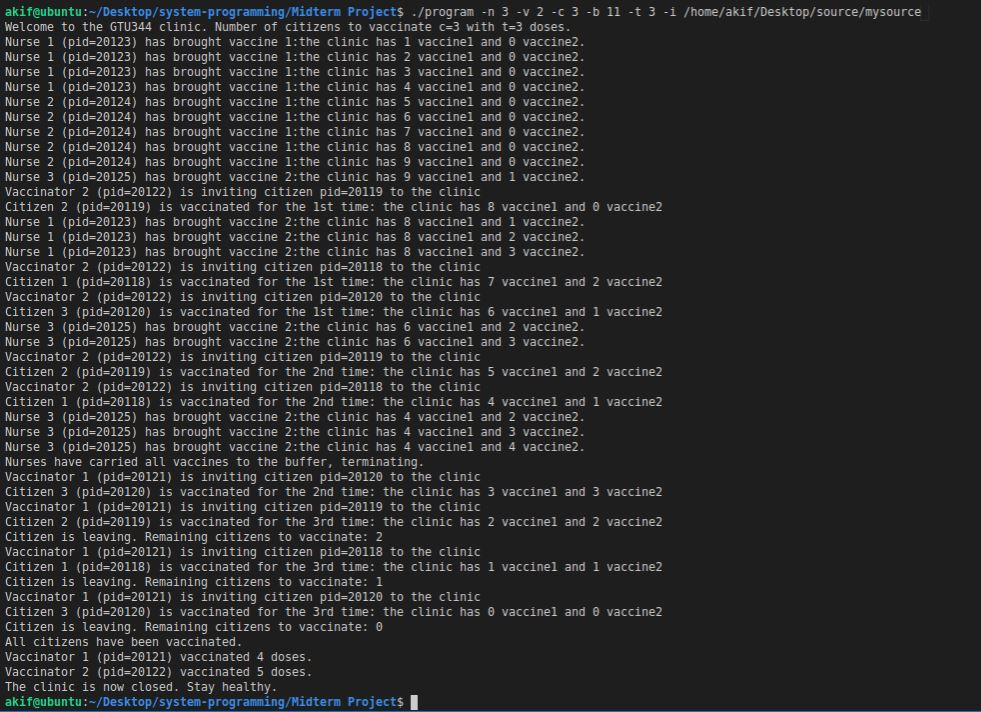
\includegraphics[width=1\textwidth, left]{result.JPG}
\caption[Optional caption]{}
\label{}
		
\end{figure}                              

\end{document}